%%%%%%%%%%%%%%%%%%%%%%%%%%%%%%%%%%%%%%%%%%%%%%%%%%%%%%%%%%%%%%%%%
%%  To create image run: (for Windows use imgconvert)
%%
%%  convert -verbose -delay 50 -loop 0 -density 300 -resize 640x480 <name>.pdf <name>.gif
%%
%%%%%%%%%%%%%%%%%%%%%%%%%%%%%%%%%%%%%%%%%%%%%%%%%%%%%%%%%%%%%%%%
\documentclass[beamer,tikz,preview]{standalone}
%\documentclass{beamer}

\setbeamertemplate{navigation symbols}{}
\usepackage{tikz}
\usepackage{color}

\tikzset{pics/.cd,
cube/.style args={#1/#2/#3/#4}{code={
\coordinate (O) at (0,0,0);
\coordinate (A) at (0,#2,0);
\coordinate (B) at (0,#2,#3);
\coordinate (C) at (0,0,#3);
\coordinate (D) at (#1,0,0);
\coordinate (E) at (#1,#2,0);
\coordinate (F) at (#1,#2,#3);
\coordinate (G) at (#1,0,#3);
\draw[black,fill=black!80] (O) -- (C) -- (G) -- (D) -- cycle;
\draw[black,fill=black!30] (O) -- (A) -- (E) -- (D) -- cycle;
\draw[black,fill=black!10] (O) -- (A) -- (B) -- (C) -- cycle;
\draw[black,fill=black!20,opacity=0.8] (D) -- (E) -- (F) -- (G) -- cycle;
\draw[black,fill=black!20,opacity=0.6] (C) -- (B) -- (F) -- (G) -- cycle;
\draw[black,fill=black!20,opacity=0.8] (A) -- (B) -- (F) -- (E) -- cycle;
\node at (0.5*#1,0.5*#2,0.5*#3) {#4};
}}}

\tikzset{pics/.cd,
lwing/.style args={#1/#2/#3/#4}{code={
\coordinate (O) at ( 0, 0, 0);
\coordinate (A) at ( 0, 0,#3);
\coordinate (B) at ( 0,#2,#3);
\coordinate (C) at ( 0,#2, 0);
\draw[black,fill=red!20] (O) -- (A) -- (B) -- (C) -- cycle;
\node at (0,0.5*#2,0.5*#3) {#4};
}}}

\tikzset{pics/.cd,
mwing/.style args={#1/#2/#3/#4}{code={
\coordinate (O) at ( 0, 0, 0);
\coordinate (A) at (#1, 0, 0);
\coordinate (B) at (#1,#2, 0);
\coordinate (C) at ( 0,#2, 0);
\draw[black,fill=green!20] (O) -- (A) -- (B) -- (C) -- cycle;
\node at (0.5*#1,0.5*#2,0) {#4};
}}}

\tikzset{pics/.cd,
rwing/.style args={#1/#2/#3/#4}{code={
\coordinate (O) at ( 0, 0, 0);
\coordinate (A) at (#1, 0, 0);
\coordinate (B) at (#1, 0,#3);
\coordinate (C) at ( 0, 0,#3);
\draw[black,fill=blue!20] (O) -- (A) -- (B) -- (C) -- cycle;
\node at (0.5*#1,0,0.5*#3) {#4};
}}}

\tikzset{pics/.cd,
    abacus2/.style args={#1/#2}{
        code={
            \draw[red] (0,0) -- (1.5,0);
            \draw[red] (0,0.25) -- (1.5,0.25);
            \foreach \u in {1,...,#1} {
                \filldraw[red] (0.1*\u,0) circle (1pt);
            }
            \foreach \u in {1,...,#2} {
                \filldraw[red] (0.1*\u,0.25) circle (1pt);
            }
        }
    } 
}

\begin{document}
\begin{frame}
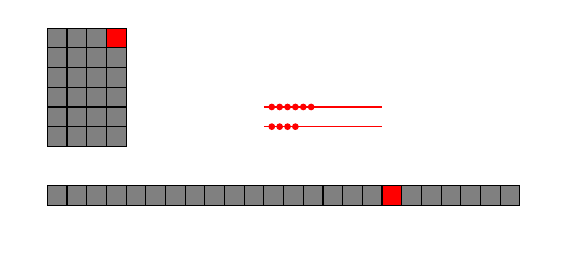
\begin{tikzpicture}
   
    \foreach \y in {1,...,6} {
        \foreach \x in {1,...,4} {
            
            \fill[color=white] (0,-0.25) rectangle (26*0.25,2);            \foreach \t in {1,...,24} {
                \draw[black,fill=gray] (0.25*\t,0) rectangle (0.25*\t+0.25,0.25);
            }
            \foreach \v in {1,...,6} {
                \foreach \u in {1,...,4} {
                    \draw[black,fill=gray] (0.25*\u,0.25*\v+0.5) rectangle (0.25*\u+0.25,0.25*\v+0.75);
                }
            }


            \pic at (3,1) {abacus2={\x/\y}};
            \draw[black,fill=red] (\x+0.25*\y-1,0) rectangle (\x+0.25*\y-0.75,0.25);
            \draw[black,fill=red] (0.25*\x,0.25*\y+0.5) rectangle (0.25*\x+0.25,0.25*\y+0.75);

            \pause

        }
    }
\end{tikzpicture}

\end{frame}

\end{document}